An isometric tensor network is a tensor network whose diagrams bonds can be consistently assigned with arrows. In particular we will look at finite tensor networks where the arrows do not form any loops. In such networks, all arrows point to a single tensor, the \textit{orthogonality center}. These networks have the very useful property that the error of local approximations around the orthogonality center can be computed locally, without contracting the full network. Let $\mathcal{N}$ be the tensor that is the result of contracting the full network, and let $\mathcal{M}$ be the tensor resulting from the contraction of a subregion of the network around the orthogonality center, where all arrows in the tensor network diagram point towards $\mathcal{M}$ (see Figure \figref{fig:isometric_tensor_network_N} for an example in tensor diagram notation). Let us now approximate the sub-network $\mathcal{M}$ by a different sub-network $\mathcal{M}^\prime$, which changes the contraction of the full network to $\mathcal{N}^\prime$ (see \figref{fig:isometric_tensor_network_N_prime}). We can compute the error $\varepsilon$ of this approximation as
\begin{equation}
\begin{split}
	\varepsilon^2 &= \lVert\mathcal{N}-\mathcal{N}^\prime\rVert^2_\text{F} \\
	&=
	\left\langle\mathcal{N}-\mathcal{N}^\prime, \mathcal{N}-\mathcal{N}^\prime\right\rangle_\text{F} \\
	&= \lVert\mathcal{N}\rVert_\text{F}^2 + \lVert\mathcal{N}^\prime\rVert_\text{F}^2 - 2\Re\left\langle\mathcal{N},\mathcal{N}^\prime\right\rangle_\text{F} \\
	&= \lVert\mathcal{M}\rVert_\text{F}^2 + \lVert\mathcal{M}^\prime\rVert_\text{F}^2 - 2\Re\left\langle\mathcal{M},\mathcal{M}^\prime\right\rangle_\text{F} \\
	&= \lVert\mathcal{M}-\mathcal{M}^\prime\rVert^2_\text{F},
\end{split}
\end{equation}
where in the fourth step we used the fact that all tensors outside of the sub-network satisfy the isometry condition. As an example, the contraction of $\langle\mathcal{N}\mathcal{N}^{\prime\dagger}\rangle_\text{F} = \langle\mathcal{M}\mathcal{M}^{\prime\dagger}\rangle_\text{F}$ is shown in Figure \figref{fig:isometric_tensor_network_norm_contraction}. As one can see, the computation of the error reduces to a contraction of the local sub-networks. This greatly simplifies the computation of optimal approximations of tensors especially for large networks, because the full network does not need to be contracted. When the tensor network represents a quantum state, this also makes it very easy to compute local expectation values, as will become clear in the next section. This is because the computation of the overlap of the wave function can be simplified to a contraction of a local environment around the orthogonality center. Additionally, approximations made by the truncated SVD \ref{eq:truncated_SVD_general} are, when performed at the orthogonality center, globally optimal for isometric tensor networks, instead of only locally optimal for non-isometric tensor networks.
\begin{figure}
	\centering
	\subcaptionbox{\label{fig:isometric_tensor_network_N}}
	{%
		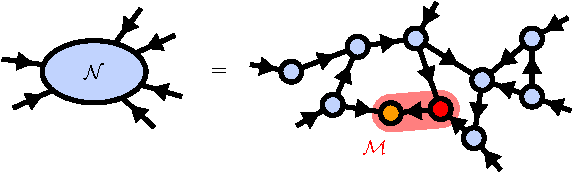
\includegraphics[scale=1]{figures/tikz/Tensor_Networks/contractions_of_isometric_tensor_networks/contractions_of_isometric_tensor_networks_a.pdf}
	}
	\par\bigskip
	\subcaptionbox{\label{fig:isometric_tensor_network_N_prime}}
	{%
		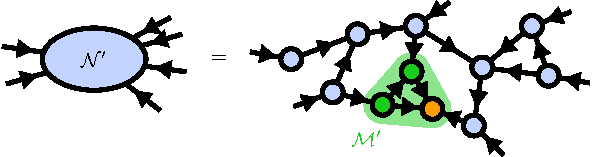
\includegraphics[scale=1]{figures/tikz/Tensor_Networks/contractions_of_isometric_tensor_networks/contractions_of_isometric_tensor_networks_b.pdf}
	}
	\par\bigskip
	\subcaptionbox{\label{fig:isometric_tensor_network_norm_contraction}}
	{%
		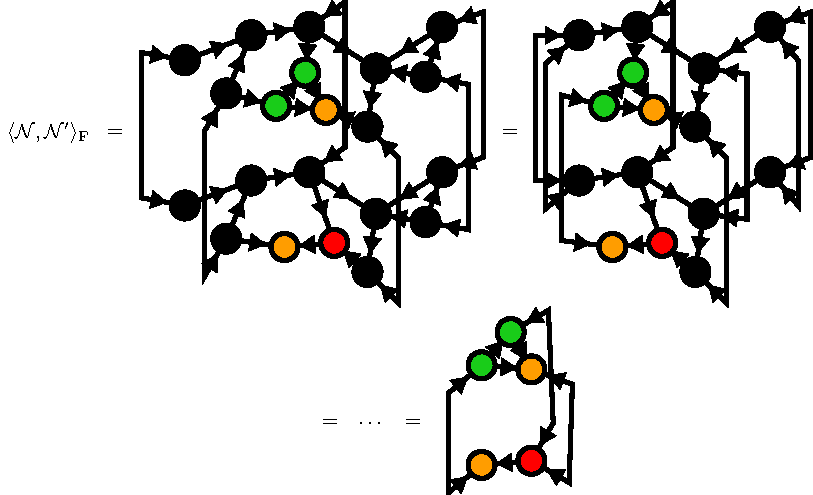
\includegraphics[scale=1]{figures/tikz/Tensor_Networks/contractions_of_isometric_tensor_networks/contractions_of_isometric_tensor_networks_c.pdf}
	}
	\caption{(a) An isometric tensor network $\mathcal{N}$ with the orthogonality center depicted in orange. The sub-network $\mathcal{M}$ is made up of all tensors in the red region. (b) The isometric tensor network $\mathcal{N}^\prime$ with an updated sub-network $\mathcal{M}^\prime$. (c) The computation of the overlap $\langle\mathcal{N},\mathcal{N}^\prime\rangle_\text{F}$ reduces to a contraction of the subregions $\langle\mathcal{M},\mathcal{M}^\prime\rangle_\text{F}$ because of the isometry condition.}
	\label{fig:isometric_tensor_network_local_approximation}
\end{figure}